% Completed operator results; tables generated from the audited cohort.
\begingroup
\renewcommand{\dbltopfraction}{0.92}
\renewcommand{\textfraction}{0.08}
\renewcommand{\dblfloatpagefraction}{0.65}
\makeatletter
\setlength{\@dblfptop}{0pt}
\setlength{\@dblfpsep}{12pt}
\setlength{\@dblfpbot}{0pt plus 1fil}
\makeatother
\raggedbottom
\section{实验评估}
\label{sec:evaluation}
本节围绕三个问题评估 Scout：约束剪枝能否减少无效探索并更早达到目标性能；分级筛选能否降低学习代价模型的评分成本；上述变化能否改善完整调优时间和最终程序性能。主实验覆盖四个算子、三种配置，共 12 组审核完成的运行、7461 次真实提交，并已完成全部原搜索赢家的独立重测。以下分别报告搜索轨迹、固定程序性能和阶段成本。

\subsection{实验设置与评价指标}
\label{sec:experiment-setup}
\paragraph{平台与负载}
实验使用 NVIDIA GeForce RTX 3050 Ti Laptop GPU（4 GiB）、TVM \texttt{0.26.dev90}、CUDA 12.6 编译工具链及 \texttt{sm\_86} 目标，精度均为 FP32。MatMul128 和 MatMul256 分别计算 $128^3$ 和 $256^3$ 矩阵乘；Conv2D 采用 NCHW 布局，输入为 $1\times16\times32\times32$，卷积核为 $32\times16\times3\times3$，步长、padding 和 groups 均为 1；Reduction 对 $128\times4096$ 输入沿第二维求和。GPU 实验串行执行，候选编译使用单工作进程，保留原实验环境与测量协议。

\paragraph{比较配置}
B 为原 MetaSchedule，C 为启用约束引导采样和分层硬筛的 CS+H，D 为进一步启用 Draft-GA 的完整 Scout。三者采用相同的调度规则定义、后处理、编译及硬件测量流程；C/D 在采样与回放阶段启用线程约束检查，D 以解析评分引导进化，并在批末调用学习代价模型。种群大小为 32，配置的 GA 迭代参数为 1，每批最多提交 10 个候选。B/C 的随机探索比例为 0.1；D 的实现将最终随机探索配额置为 0。因此，C/D 比较反映分级筛选及候选选择策略的整体变化，尚未单独控制随机探索的影响。

Draft 入围比例为 $0.25$，且入围数不低于本批候选需求。对于需求为 10 的常规批次，$K=\max(10,\lceil0.25\times32\rceil)=10$，批末学习模型主要对这 10 个候选重排。这组设置主要检验将高频评分移出进化循环的成本变化；入围集合大小对候选保留率的影响仍需另外验证。

\paragraph{预算与反馈历史}
每组提交上限为 800，失败同样消耗预算，不以重复提交填满上限。九组矩阵乘与卷积实验均完成 800 次提交；归约三组在搜索无法继续产生候选后正常终止，B/C/D 实际提交数分别为 85/88/88，按真实终点报告。所有提交均得到有限测量结果，并通过相应数值检查。Conv2D/C 由审核一致的 298 次历史提交接续完成其余 502 次；活动 Tune 时间累加历史与接续阶段，暂停间隔及 456.91 s 的状态重建时间单列，不计入活动搜索曲线。该口径衡量实际调优工作时间，不等于包含暂停的日历时间。

搜索 seed 固定为 20261011。各配置独立维护 XGBoost 模型和测量历史，模型的 \texttt{warmup\_samples=0}；收到新增有效反馈后，使用全部累计样本重新拟合，配置之间不共享反馈。TVM 使用 CUDA 事件计时，设置为 \texttt{number=3}、\texttt{repeat=1}、\texttt{min\_repeat\_ms=100}，计时器按最小测量时长调整执行次数。独立重测固定各组原搜索选出的最佳实测合法候选，重新编译后每轮预热 100 次，执行 3 轮、每轮 10 个技术样本，报告中位数及四分位区间；重测不重新挑选赢家，也不回填搜索曲线。

\paragraph{统一目标与计时口径}
搜索曲线在每批完整反馈可用后更新，分别以累计真实提交数和活动 Tune 墙钟时间为横轴。设 $L_B^{\mathrm{end}}$ 为 B 在实际运行终点获得的最佳观测延迟，$L_m(t)$ 为配置 $m$ 在时刻 $t$ 已获得的最佳延迟，定义
\begin{equation}
T_m(\epsilon)=\min\{t:L_m(t)\le(1+\epsilon)L_B^{\mathrm{end}}\}.
\label{eq:target-time}
\end{equation}
主比较采用严格目标 $\epsilon=0$，同时报告 $\epsilon=0.01$ 和 $0.05$ 的容差目标。达标加速比为 $T_B(\epsilon)/T_m(\epsilon)$，分子同样取 B 首次达标的时间。未达到目标记为 NR，并报告实际运行总时长。阈值比例预先固定，绝对阈值由 B 终点确定，因此这是回顾性的统一质量比较。首次达到各自最终最佳值的位置用于描述平台出现时间，不用于比较不同质量水平下的调优加速。

\subsection{最终程序性能}
\label{sec:operator-performance}
表~\ref{tab:operator800-endpoints} 给出全部 12 组的搜索终点。C 在 MatMul128 上与 B 接近，在 Conv2D 上取得更低的观测延迟；MatMul256 和 Reduction 则由 B 获得更低的终点延迟。D 在四个算子上的终点均高于 B，表明减少学习模型评分次数本身并不能保证提高候选质量。

\begin{table}[t]
\centering
\caption{搜索终点的最佳观测延迟（$\mu$s）。最后一列依次为 B/C/D 的真实提交数；800 为上限，归约按实际提前终止点报告。}
\label{tab:operator800-endpoints}
\small
\setlength{\tabcolsep}{3pt}
% Generated by experiments/build_operator800_paper_tables.py.
\begin{tabular}{@{}lrrrr@{}}
\toprule
算子 & B & C & D & 提交数 B/C/D \\
\midrule
MatMul128 & 27.246 & 27.253 & 27.717 & 800/800/800 \\
MatMul256 & 26.424 & 29.810 & 29.458 & 800/800/800 \\
Conv2D & 29.200 & 28.245 & 29.705 & 800/800/800 \\
Reduction & 31.126 & 31.788 & 35.501 & 85/88/88 \\
\bottomrule
\end{tabular}

\end{table}

\begin{table*}[t]
\centering
\caption{全部原搜索赢家的独立重测。每组 30 个技术样本，延迟单位为 $\mu$s；相对性能为同算子 B 的中位数除以对应中位数，大于 1 表示快于 B。PyTorch 为单独进程中的框架参考，不参与调优加速比计算。}
\label{tab:operator800-retiming}
\small
\setlength{\tabcolsep}{6pt}
% Generated by experiments/build_operator800_paper_tables.py.
\begin{tabular*}{0.92\textwidth}{@{\extracolsep{\fill}}lrrr@{}}
\toprule
算子 / 配置 & 中位数 & [P25, P75] & 相对 B 的性能 \\
\midrule
MatMul128 / B & 29.225 & [28.791, 30.650] & 1.000 \\
MatMul128 / C & 28.873 & [28.143, 30.051] & 1.012 \\
MatMul128 / D & 31.418 & [30.669, 32.089] & 0.930 \\
MatMul128 / PyTorch & 13.831 & [12.879, 14.982] & -- \\
\midrule
MatMul256 / B & 28.288 & [27.399, 29.449] & 1.000 \\
MatMul256 / C & 30.715 & [29.765, 31.304] & 0.921 \\
MatMul256 / D & 31.315 & [30.860, 33.628] & 0.903 \\
MatMul256 / PyTorch & 16.305 & [15.576, 17.232] & -- \\
\midrule
Conv2D / B & 28.563 & [28.249, 29.257] & 1.000 \\
Conv2D / C & 29.383 & [29.105, 30.004] & 0.972 \\
Conv2D / D & 29.018 & [28.506, 29.617] & 0.984 \\
Conv2D / PyTorch & 25.585 & [24.236, 28.562] & -- \\
\midrule
Reduction / B & 28.598 & [27.646, 29.575] & 1.000 \\
Reduction / C & 28.562 & [27.867, 29.464] & 1.001 \\
Reduction / D & 32.862 & [32.094, 33.622] & 0.870 \\
Reduction / PyTorch & 10.605 & [10.484, 11.043] & -- \\
\bottomrule
\end{tabular*}

\end{table*}

独立重测结果见表~\ref{tab:operator800-retiming}。C 相对 B 的性能比分别为 1.012、0.921、0.972 和 1.001；D 分别为 0.930、0.903、0.984 和 0.870。Conv2D/C 的搜索最小值虽低于 B，其固定赢家的重测中位数仍高于 B，说明搜索中的单次最小值与程序重测性能需要分开考察。技术重复描述所选程序的计时波动，不构成多个独立搜索 seed 的证据。

PyTorch 参考使用 \texttt{2.11.0+cu128}（CUDA 12.8），关闭 TF32，输入常驻 GPU；矩阵乘和归约复用输出缓冲区，卷积使用框架原生输出分配。其 CUDA 事件区间包含 Python 发射间隔，且运行栈与 TVM 的 CUDA 12.6 编译工具链不同。四个参考中位数分别为 13.831、16.305、25.585 和 10.605 $\mu$s，用于定位当前程序性能，不作为学习模型或剪枝策略的消融对照。

\subsection{搜索收敛与达到目标性能的时间}
\label{sec:search-quality}
图~\ref{fig:operator800-convergence} 将四个算子的 B/C/D 收敛曲线合为一张主图。左列按提交次数裁去三种方法均不再改善的共同平台尾部，中列放大前 100 次提交，右列展示对应的活动 Tune 时间。每个算子的三种方法使用相同显示范围和纵轴尺度，左右两列均保留全部已观测到的性能改善。截尾仅用于事后展示，不代表运行时采用了提前停止规则。所有曲线均为批末可用结果的阶梯线，不平滑、不补足提前终止的提交，也不以独立重测改变历史轨迹；完整预算曲线另行保留。表~\ref{tab:operator800-convergence} 同时列出首次自身最佳位置、统一目标时间和总调优成本。

\begin{figure*}[p]
\centering
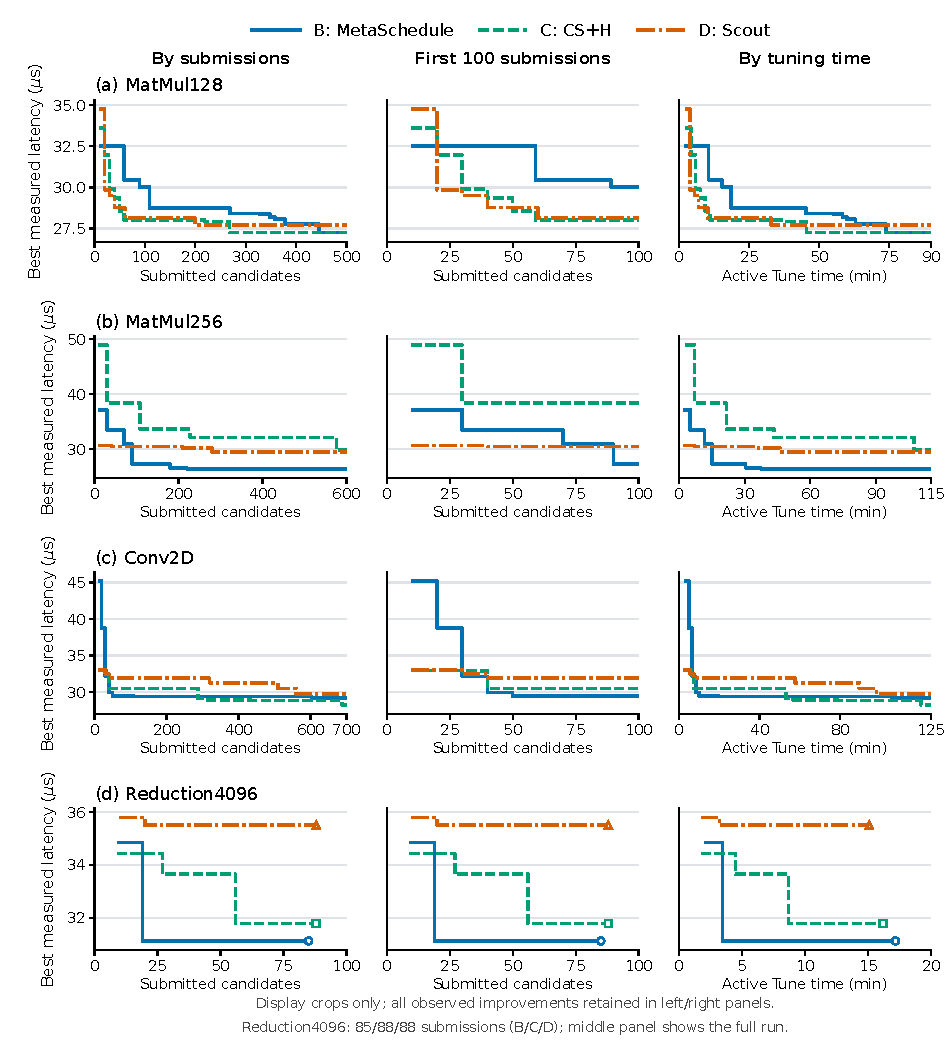
\includegraphics[width=\textwidth]{figures/operator800_20261011_cohort/paper_main_convergence_zoomed/operator800_main_convergence.pdf}
\caption{算子收敛与前 100 次放大。左列依次截至 500/600/700/100 次提交，右列依次截至 90/115/125/20 min，三种方法共用显示范围；左右两列保留全部已观测改善。纵轴为累计最佳延迟。B/C/D 分别为 MetaSchedule、CS+H、完整 Scout。空心点表示实际终点；归约仅 85/88/88 次，中列覆盖完整运行。Conv2D/C 不计暂停与状态重建。单搜索 seed，重测不回填。}
\label{fig:operator800-convergence}
\end{figure*}

\begin{table*}[t]
\centering
\caption{全部运行的收敛位置与统一目标时间，单位为 min。自身最佳位置取完整反馈后的批末；严格、+1\%、+5\% 目标均相对于同算子 B 的搜索终点。NR 表示截至本行总调优时间仍未达到目标。}
\label{tab:operator800-convergence}
\small
\setlength{\tabcolsep}{4pt}
% Generated by experiments/build_operator800_paper_tables.py.
\begin{tabular*}{\textwidth}{@{\extracolsep{\fill}}lrrrrrr@{}}
\toprule
算子 / 配置 & \shortstack{自身最佳\\提交数} & \shortstack{自身最佳\\时间} & \shortstack{严格\\目标} & \shortstack{+1\%\\目标} & \shortstack{+5\%\\目标} & 总调优 \\
\midrule
MatMul128 / B & 446 & 74.08 & 74.08 & 74.08 & 45.37 & 134.01 \\
MatMul128 / C & 268 & 45.65 & NR & 45.65 & 9.39 & 135.21 \\
MatMul128 / D & 200 & 32.84 & NR & NR & 10.29 & 130.31 \\
\midrule
MatMul256 / B & 220 & 37.22 & 37.22 & 30.47 & 15.17 & 136.48 \\
MatMul256 / C & 576 & 107.36 & NR & NR & NR & 150.60 \\
MatMul256 / D & 280 & 46.04 & NR & NR & NR & 132.57 \\
\midrule
Conv2D / B & 603 & 105.57 & 105.57 & 10.01 & 8.36 & 140.23 \\
Conv2D / C & 688 & 120.02 & 53.06 & 53.06 & 7.56 & 139.23 \\
Conv2D / D & 560 & 98.10 & NR & NR & 89.50 & 138.00 \\
\midrule
Reduction / B & 19 & 3.45 & 3.45 & 3.45 & 3.45 & 17.19 \\
Reduction / C & 56 & 8.71 & NR & NR & 8.71 & 16.22 \\
Reduction / D & 20 & 3.23 & NR & NR & NR & 15.11 \\
\bottomrule
\end{tabular*}

\end{table*}

\paragraph{剪枝配置的达标收益}
Conv2D 中，C 在 53.06 min 达到 B 的严格终点目标，B 首次达到该目标需要 105.57 min，因此 C 取得 $1.99\times$ 达标加速，对应耗时减少 49.7\%。C 随后继续改善，在 120.02 min 获得自身最佳观测值 $28.245\,\mu$s。完整提交上限下，C/B 总时间分别为 139.23/140.23 min；提前获得目标性能的收益明显大于跑完全部提交后的总时间差异。

MatMul128 中，C 的终点为 $27.253\,\mu$s，与 B 的 $27.246\,\mu$s 相差约 0.025\%，未满足严格目标；在 +1\% 目标下，C/B 分别需要 45.65/74.08 min，获得 $1.62\times$ 达标加速，耗时减少 38.4\%。在 +5\% 目标下，两者分别需要 9.39/45.37 min。MatMul256/C 则在三个目标下均未达标；Reduction/C 仅达到 +5\% 目标，且晚于 B。这些差异表明剪枝对候选数量的改善尚不能推导为所有负载上的收敛加速。

\paragraph{分级筛选的质量与时间权衡}
D 在四个算子上均未达到严格及 +1\% 目标。MatMul128/D 虽在 32.84 min 获得自身最终最佳值，但其延迟比 B 高约 1.73\%；Conv2D/D 在 +5\% 目标下需要 89.50 min，也晚于 B 的 8.36 min。因此，较早出现自身平台并不表示在相同质量下更快收敛。矩阵乘与卷积的 D 相对 B 总调优时间分别减少 2.76\%、2.87\% 和 1.59\%，但均伴随较差的终点或重测性能；归约的实际提交数还不同，需连同终止位置和程序质量解读。

\FloatBarrier
\subsection{约束剪枝对无效探索的影响}
\label{sec:invalid-exploration}
表~\ref{tab:invalid-exploration} 比较 B/C 的内部生成尝试、\texttt{VerifyGPUCode} 失败和后处理通过率。内部生成次数不等于硬件提交数；通过率以实际通过后处理的数量除以生成次数计算，其他阶段也可能拒绝候选，故不使用一减 Verify 失败率替代。

\begin{table*}[t]
\centering
\caption{约束剪枝对内部候选的影响。每种配置依次列出生成数、Verify 失败数及后处理通过率。$\dagger$：Conv2D/C 为接续运行，原生内部计数包含状态重建期间的工作，不能视为与活动 Tune 时间严格对齐的增量计数。}
\label{tab:invalid-exploration}
\small
\setlength{\tabcolsep}{4pt}
% Generated by experiments/build_operator800_paper_tables.py.
\begin{tabular*}{\textwidth}{@{\extracolsep{\fill}}lrrrrrr@{}}
\toprule
 & \multicolumn{3}{c}{B：MetaSchedule} & \multicolumn{3}{c}{C：CS+H} \\
算子 & 生成数 & Verify 失败 & 通过率 & 生成数 & Verify 失败 & 通过率 \\
\midrule
MatMul128 & 22018 & 17128 & 22.2\% & 7436 & 1950 & 70.3\% \\
MatMul256 & 25529 & 20602 & 19.3\% & 9983 & 4631 & 51.7\% \\
Conv2D$^{\dagger}$ & 19841 & 14890 & 25.0\% & 7463 & 1944 & 71.1\% \\
Reduction & 760 & 0 & 100.0\% & 759 & 0 & 100.0\% \\
\bottomrule
\end{tabular*}

\end{table*}

在 MatMul128 上，C 将生成次数从 22018 减至 7436，减少 66.2\%；Verify 失败从 17128 减至 1950，减少 88.6\%；后处理通过率由 22.2\% 升至 70.3\%。MatMul256 的生成次数和 Verify 失败分别减少 60.9\% 和 77.5\%，通过率由 19.3\% 升至 51.7\%。Conv2D 的原生累计记录同样呈现更少生成与失败、更高通过率的趋势，但含重建工作，应与其活动时间分开使用。Reduction 的基线 Verify 失败已经为零，B/C 通过率均为 100\%，缺少同类非法候选可供剪除。

这些结果支持线程约束前移能减少相关负载的无效内部探索；本组比较尚未分离 CS 与 H 的各自贡献。候选数量变化也不等于 Search 时间同比减少：例如 MatMul128 的 B/C 搜索阶段分别耗时 17.07/17.95 min，额外约束分析和不同搜索轨迹共同影响实际成本。

\subsection{分级筛选与学习代价模型成本}
\label{sec:ga-density}
表~\ref{tab:operator800-model-history} 汇总全部运行的模型反馈历史和评分成本。评分时间包围 \texttt{CostModel::Predict}，包含特征提取、数据整理与预测，不仅是树模型推理；模型更新时间包含特征、验证与重新拟合，是反馈回调的子项。

\begin{table*}[t]
\centering
\caption{学习代价模型与 Draft 的累计成本，时间单位为 s。评分输入按调用累计，可重复包含同一候选；历史样本为实际测量反馈数，更新回调次数含无新增反馈的空批次。$\dagger$：Conv2D/C 的模型评分输入数和评分时间包含状态重建，表中保留原值，不据此计算活动调优期间的 C/D 净节省。}
\label{tab:operator800-model-history}
\label{tab:draft-scoring}
\small
\setlength{\tabcolsep}{4pt}
% Generated by experiments/build_operator800_paper_tables.py.
\begin{tabular*}{\textwidth}{@{\extracolsep{\fill}}lrrrrrr@{}}
\toprule
算子 / 配置 & \shortstack{累计\\样本} & \shortstack{更新回调\\次数} & \shortstack{模型评分\\输入数} & \shortstack{模型评分\\时间} & \shortstack{模型更新\\时间} & \shortstack{Draft\\时间} \\
\midrule
MatMul128 / B & 800 & 81 & 5184 & 27.915 & 22.434 & -- \\
MatMul128 / C & 800 & 81 & 5184 & 27.551 & 25.076 & -- \\
MatMul128 / D & 800 & 80 & 800 & 4.314 & 22.541 & 0.927 \\
\midrule
MatMul256 / B & 800 & 81 & 5184 & 28.240 & 28.428 & -- \\
MatMul256 / C & 800 & 81 & 5184 & 30.941 & 30.582 & -- \\
MatMul256 / D & 800 & 80 & 800 & 4.256 & 28.490 & 0.789 \\
\midrule
Conv2D / B & 800 & 81 & 5184 & 107.516 & 40.204 & -- \\
Conv2D / C$^{\dagger}$ & 800 & 82 & 5248 & 99.787 & 42.743 & -- \\
Conv2D / D & 800 & 80 & 800 & 16.845 & 37.844 & 1.718 \\
\midrule
Reduction / B & 85 & 16 & 1088 & 1.414 & 3.814 & -- \\
Reduction / C & 88 & 16 & 1088 & 1.319 & 3.454 & -- \\
Reduction / D & 88 & 15 & 88 & 0.114 & 3.296 & 0.041 \\
\bottomrule
\end{tabular*}

\end{table*}

MatMul128 和 MatMul256 中，D 将学习模型评分输入数均由 C 的 5184 降至 800，减少 84.6\%；评分时间分别从 27.551/30.941 s 降至 4.314/4.256 s，减少 84.3\%/86.2\%。归约中，评分输入数从 1088 降至 88，评分时间从 1.319 s 降至 0.114 s，减少 91.4\%。对应 Draft 已记录耗时分别为 0.927、0.789 和 0.041 s。这些结果说明解析评分替代高频学习模型调用能够降低评分环节成本。Draft 计时尚未完整覆盖归档排序、候选收集与堆插入，因此不能将两类计时之差直接作为系统净收益。

九组 800 次提交实验均保留 800 个历史样本，归约三组保留 85/88/88 个样本；D 并未减少实际反馈样本量，也未改变非空反馈批次使用累计历史重新拟合的训练策略。归约三组的更新回调数为 16/16/15，其中实际新增反馈批次为 12/12/11。模型更新回调耗时在矩阵乘与卷积中为 22.4--42.7 s，归约中为 3.3--3.8 s。因此，当前证据支持降低评分及相关特征提取工作量，不能据此声称降低模型训练复杂度。

\begin{table*}[t]
\centering
\caption{全部 12 组活动 Tune 阶段成本（min）。测量与反馈包含 runner 调度和数值检查；模型更新包含在回调中，不重复相加。总调优不含 Tune 前准备、独立重测和接续状态重建，归约按实际终止点统计；四舍五入可能造成小计差异。}
\label{tab:operator800-phases}
\small
\setlength{\tabcolsep}{4pt}
% Generated by experiments/build_operator800_paper_tables.py.
\begin{tabular*}{\textwidth}{@{\extracolsep{\fill}}lrrrrrr@{}}
\toprule
算子 / 配置 & 搜索 & 编译 & 测量与反馈 & 回调 & 其他 & 总调优 \\
\midrule
MatMul128 / B & 17.07 & 91.08 & 4.99 & 20.45 & 0.42 & 134.01 \\
MatMul128 / C & 17.95 & 91.37 & 4.97 & 20.49 & 0.42 & 135.21 \\
MatMul128 / D & 16.51 & 87.91 & 5.01 & 20.45 & 0.43 & 130.31 \\
\midrule
MatMul256 / B & 19.40 & 90.99 & 5.15 & 20.55 & 0.39 & 136.48 \\
MatMul256 / C & 23.88 & 100.33 & 5.33 & 20.59 & 0.48 & 150.60 \\
MatMul256 / D & 21.53 & 84.93 & 5.16 & 20.55 & 0.40 & 132.57 \\
\midrule
Conv2D / B & 18.23 & 95.38 & 5.38 & 20.75 & 0.49 & 140.23 \\
Conv2D / C & 18.51 & 94.52 & 4.89 & 20.80 & 0.51 & 139.23 \\
Conv2D / D & 16.96 & 94.37 & 5.47 & 20.71 & 0.48 & 138.00 \\
\midrule
Reduction / B & 0.05 & 13.85 & 0.63 & 2.20 & 0.47 & 17.19 \\
Reduction / C & 0.04 & 12.92 & 0.62 & 2.27 & 0.37 & 16.22 \\
Reduction / D & 0.03 & 11.86 & 0.61 & 2.26 & 0.35 & 15.11 \\
\bottomrule
\end{tabular*}

\end{table*}

作为补充，独立的 32 次提交 MatMul128 初步实验曾比较 GA1/GA4：C 的模型评分输入由 512 增至 1280，D 均为 64；C/D 评分时间从 2.561/0.333 s 变为 6.427/0.330 s。该小预算结果说明内部搜索增密会放大学习模型评分成本，未证明增加代数能够改善最终程序质量，也不与 800 上限的主实验合并计算收益。

\subsection{完整调优成本与实验范围}
\label{sec:cost-and-feedback}
表~\ref{tab:operator800-phases} 将活动 Tune 时间分为互不重叠的阶段。矩阵乘与卷积中，编译是主要成本，耗时为 84.93--100.33 min；搜索为 16.51--23.88 min，反馈回调约为 20.45--20.80 min。归约的编译耗时为 11.86--13.85 min，搜索仅约 0.03--0.05 min。因而，减少数秒至数十秒的评分调用，尚不足以显著改变当前以编译为主的完整预算成本。

\paragraph{证据边界与后续验证}
\label{sec:end-to-end}
上述结论来自单块 GPU、一个搜索 seed 和四个固定形状的 FP32 算子。30 次技术重测不能替代多 seed 搜索，归约提前终止也不能解释为已完成 800 次测量。完整模型调优目前尚无完成的三配置对照，不将单算子结果或中断模型运行作为端到端收益证据。后续需补充多 seed、其他设备、完整模型，以及固定随机探索比例和独立候选池下的排序与保留率实验，以检验分级筛选在程序质量、入围比例和搜索密度之间的权衡。
\FloatBarrier
\endgroup
